\documentclass{article}
\title{Vector Spaces}
\author{Carl Schader}
\date{}

\usepackage{amsmath}
\usepackage{graphicx}

\begin{document}
	\maketitle
	\tableofcontents
	\newpage

	\section{$\mathbf{R}^n$ and $\mathbf{C}^n$}
	\subsection{Complex Numbers}
	\subsubsection{Definition of Complex Numbers}
	\begin{itemize}
		\item A \textbf{complex number} is an ordered pair $(a, b)$, where $a, b \in \mathbf{R}$, and can be written as $a + bi$.
		\item The set of all complex numbers is denoted by $\mathbf{C}$:
		\begin{equation*}
			\mathbf{C} = \{ a + bi : a, b \in \mathbf{R} \}
		\end{equation*}
		\item \text{Addition and Multiplication of Complex Numbers} on $\mathbf{C}$ are defined by:
		\begin{align*}
			(a + bi) + (c + di) &= (a + c) + (b + d)i\\
			(a + bi)(c + di) &= (ac - bd) + (ad + bc)i
		\end{align*}
		where $a,b,c,d \in \mathbf{R}$.
		\item $a + 0i$ is denoted as $a$.\\
			$0 + bi$ is denoted as $bi$.\\
		\item $\mathbf{R} \subset \mathbf{C}$
		\item $i = \sqrt{-1}$.
	\end{itemize}
	
	\subsubsection{Properties of Complex Arithmetic}
	\begin{itemize}
		\item \textbf{commutativity}
		\begin{equation*}
			\alpha + \beta = \beta + \alpha \text{ and } \alpha\beta = \beta\alpha \text{ for all } \alpha,\beta\in\mathbf{C};
		\end{equation*}

		\item \textbf{associativity}
		\begin{equation*}
			(\alpha + \beta) + \lambda = \alpha + (\beta + \lambda) \text{ and } (\alpha\beta)\lambda = \alpha(\beta\lambda) \text{ for all } \alpha,\beta\in\mathbf{C};
		\end{equation*}

		\item \textbf{identities}
		\begin{equation*}
			\lambda + 0 = \lambda \text{ and } \lambda 1 = \lambda \text{ for all } \lambda \in \mathbf{C}; 
		\end{equation*}

		\item \textbf{additive inverse}
		\begin{equation*}
			\text{for every } \alpha\in\mathbf{C} \text{ with } \alpha\neq 0 \text{, there exists a unique } \beta\in\mathbf{C} \text{ such that } \alpha + \beta = 0;
		\end{equation*}

		\item \textbf{multiplicative inverse}
		\begin{equation*}
			\text{for every } \alpha\in\mathbf{C} \text{ with } \alpha\neq 0 \text{, there exists a unique } \beta\in\mathbf{C} \text{ such that } \alpha\beta = 1;
		\end{equation*}

		\item \textbf{distributive property}
		\begin{equation*}
			\lambda(\alpha + \beta) = \lambda\alpha + \lambda\beta \text{ for all } \lambda,\alpha,\beta\in\mathbf{C}.
		\end{equation*}
	\end{itemize}

	\subsubsection{Subtraction and Division of Complex Numbers}
	Let $\alpha,\beta\in\mathbf{C}$.
	\begin{itemize}
		\item Let $-\alpha$ denote the additive inverse of $\alpha$. Thus $-\alpha$ is the unique complex number such that
		\begin{equation*}
			\alpha + (-\alpha) = 0.
		\end{equation*}
		\item \textbf{Subtraction} on $\mathbf{C}$ is defined by
		\begin{equation*}
			\beta - \alpha = \beta + (-\alpha).
		\end{equation*}
		\item For $\alpha\neq0$, let $1/\alpha$ denote the multiplicative inverse of $\alpha$. Thus $1/\alpha$ is the unique complex number such that
		\begin{equation*}
			\alpha(1/\alpha) = 1.
		\end{equation*}
		\item \textbf{Division} on $\mathbf{C}$ is defined by
		\begin{equation*}
			\beta/\alpha = \beta(1/\alpha).
		\end{equation*}
	\end{itemize}

	\subsubsection{Notation $\mathbf{F}$}
	Throughout this book, $\mathbf{F}$ stands for either $\mathbf{R}$ or $\mathbf{C}$. The letter $\mathbf{F}$ is used because $\mathbf{R}$ and $\mathbf{C}$ are examples of \textbf{fields}. Elements of $\mathbf{F}$ are also called \textbf{scalars}.

	\subsection{Lists}
	\subsubsection{Definition of Lists}
	Suppose $n$ is a nonnegative integer. A \textbf{list} of \textbf{length} $n$ is an \textbf{ordered} collection of $n$ elements (not necessarily numbers) seperated by commas and surrounded by parentheses. A list must also have a finite length. A list of length $n$, or an \textbf{n-tuple}, looks like:
	\begin{equation*}
		\left( x_1, ..., x_n \right).
	\end{equation*} 
	Two lists are equal if and only if they have the same length and the same elements in the same order. Lists differ from sets in that order matters and repititions are not meaningless.

	\subsubsection{Definition of $\mathbf{F}^n$}
	$\mathbf{F}^n$ is the set of all lists of length $n$ made up with elements of $\mathbf{F}^n$:
	\begin{equation*}
		\mathbf{F}^n = \{ \left( x_1, ..., x_n \right) : x_j \in \mathbf{F} \text{ for } j=1,...,n \}.
	\end{equation*}
	If $\mathbf{F} = \mathbf{R}$ and $n$ equals $2$ or $3$, then this defintion of $\mathbf{F}^n$ is the same as $\mathbf{R}^2$ or $\mathbf{R}^3$. Lists in $\mathbf{F}^n$ are also called vectors.

	\subsubsection{Addition in $\mathbf{F}^n$}
	\begin{equation*}
		(x_1, ..., x_n) + (y_1, ..., y_n) = (x_1 + y_1, ..., x_n + y_n)
	\end{equation*} 

	\subsubsection{Commutativity of Addition in $\mathbf{F}^n$}
	If $x,y\in\mathbf{F}^n$, then $x + y = y + x$.

	\subsubsection{Definition of the $0$ List}
	Let $0$ denote the list of length $n$ whose coordinates are all $0$:
	\begin{equation*}
		0 = (0, ..., 0).
	\end{equation*}

	\subsubsection{Geometric Interpretation of Vectors}
	\begin{itemize}
		\item We can think of lists or vectors not just as points but also as arrows in Euclidean spaces.
		\item We can translate a vector without changing its length or direction and still think of it as the same vector.
		\item Addition of vectors can be thought of as taking two vectors and translating one so that its start touches the end of the other and drawing a new vector from the begining of the chain to the end of the chain.
	\end{itemize}

	\begin{figure}[h!]
	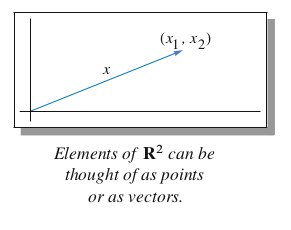
\includegraphics{geometric-interpretation-of-vectors-1.png}
	\end{figure}
	
	\begin{figure}[h!]
	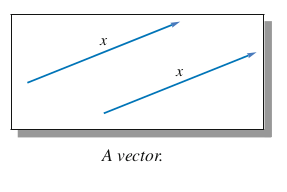
\includegraphics{geometric-interpretation-of-vectors-2.png}
	\end{figure}

	\begin{figure}[h!]
	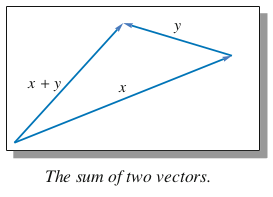
\includegraphics{geometric-interpretation-of-vectors-3.png}
	\end{figure}

	\subsubsection{Additive Inverse in $\mathbf{F}^n$}
	For $x\in\mathbf{F}^n$, the \textbf{additive inverse} of $x$, denoted $-x$, is the vector $-x\in\mathbf{F}^n$ such that
	\begin{equation*}
		x + \left( -x \right) = 0.
	\end{equation*}
	In other words, if $x = \left( x_1, ..., x_n \right)$, then $-x = \left( -x_1, ..., -x_n \right)$.\\
	The vector $-x$ is parallel to $x$ and has the same length but facing the opposite direction.

	\subsubsection{Scalar Multiplication in $\mathbf{F}^n$}
	The \textbf{product} of a number $\lambda$ and a vector $\mathbf{F}^n$ is computed by multiplying each element or coordinate of the vector by $\lambda$:
	\begin{equation*}
		\lambda\left( x_1, ..., x_2 \right) = \left( \lambda x_1, ..., \lambda x_n \right);
	\end{equation*}
	here $\lambda\in\mathbf{F}$ and $(x_1, ..., x_n)\in \mathbf{F}^n$.
	\begin{figure}[h!]
	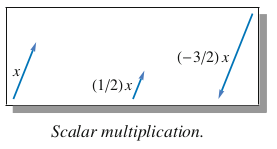
\includegraphics{scalar-vector-multiplication.png}
	\end{figure}

	\section{Definition of Vector Space}
	\subsection{Addition and Scalar Multiplication on a Set}
	\begin{itemize}
		\item An \textbf{addition} on a set $V$ is a function that assigns an element $u + v \in V$ to each pair of elements $u, v \in V$.
		\item A \textbf{scalar multiplication} on a set $V$ is a function that assigns an element $\lambda v \in V$ to each $\lambda \in \mathbf{F}$ and each $v \in V$.
	\end{itemize}

	\subsection{Vector Space}
	A \textbf{vector space} is a set $V$ along with an addition on $V$ and a scalar multiplication on $V$ such that the following properties hold:
	\begin{itemize}
		\item \textbf{commutativity}
		\begin{equation*}
			u + v = v + u \text{ for all } u,v\in V;
		\end{equation*}

		\item \textbf{associativity}
		\begin{equation*}
			(u + v) + w = u + (v + w) \text{ and } (ab)v = a(bv) \text{ for all } u,v,w\in V \text{ and all } a,b\in\mathbf{F};
		\end{equation*}

		\item \textbf{additive identity}
		\begin{equation*}
			\text{there exists an element } 0\in V \text{ such that } v + 0 = v \text{ for all } v\in V;
		\end{equation*}

		\item \textbf{additive inverse}
		\begin{equation*}
			\text{for every } v\in V \text{ there exists } w\in V \text{ such that } v + w = 0;
		\end{equation*}

		\item \textbf{multiplicative identity}
		\begin{equation*}
			1v = v\text{ for all } v\in V;
		\end{equation*}

		\item \textbf{distributive properties}
		\begin{equation*}
			a(u + v) = au + av \text{ and } (a + b)v = av + bv \text{ for all } a,b\in \mathbf{F} \text{ and all } u,v\in V;
		\end{equation*}
		Elements of a vector space are called \textbf{vectors} or \textbf{points}.
	\end{itemize}

	\subsection{Real Vector Space vs. Complex Vector Space}
	Scalar multiplication in a vector space depends on $\mathbf{F}$. Thus when we need to specify we say that $V$ is a vector space over $\mathbf{F}$.
	\begin{itemize}
		\item A vector space over $\mathbf{R}$ is called a real vector space.
		\item A vector space over $\mathbf{C}$ is called a complex vector space.
	\end{itemize}

	\subsection{$\mathbf{F}^S$}
	\begin{itemize}
		\item If $S$ is a set, then $\mathbf{F}^S$ denotes the set of functions $f:S\to\mathbf{F}$.
		\item For $f,g\in\mathbf{F}^S$, the sum $f + g\in\mathbf{F}^S$ is the function defined by
		\begin{equation*}
			(f + g)(x) = f(x) + g(x)
		\end{equation*}
		for all $x\in S$.
		\item For $\lambda\in\mathbf{F}$ and $f\in\mathbf{F}^S$, the product $\lambda f\in\mathbf{F}^S$ is the function defined by
		\begin{equation*}
			(\lambda f)(x) = \lambda f(x)
		\end{equation*}
		for all $x\in S$.
	\end{itemize}

	\section{Subspaces}
	\subsection{Definition Subspace}
	A subset $U$ of a vector space $V$ is called a \textbf{subspace}, or \textbf{linear subsapace}, of $V$ if $U$ is also a vector space (using the smae addition and scalar multiplication as on $V$).

	\subsection{Conditions for a Subspace}
	A subset $U$ of vector space $V$ is a subspace of $V$ if and only if $U$ satisfies the following three conditions:
	\begin{itemize}
		\item\textbf{additive identity}
		\begin{equation*}
			\text{if } 0 \text{ is the additive identity of } V \text{, then } 0\in U;
		\end{equation*}
		\item\textbf{closed under addition}
		\begin{equation*}
			u,w\in U \text{ implies } u+ w \in U;
		\end{equation*}
		\item\textbf{closed under scalar multiplication}
		\begin{equation*}
			a\in\mathbf{F} \text{ and } u \in U \text{ implies } au\in U.
		\end{equation*}
	\end{itemize}

	\subsection{Subspaces of $\mathbf{R}^2$}
	All the subspaces of $\mathbf{R}^2$ are $\{0\}$, $\mathbf{R}^2$, and all the lines in $\mathbf{R}^2$ through the origin.

	\subsection{Sums of Subspaces}
	\subsubsection{Sum of Subsets}
	Suppose $U_1, ..., U_m$ are all subsets of $V$. The \textbf{sum} of $U_1, ..., U_m$, denoted $U_1 + ... + U_m$, is the set of all possible sums of elements of $U_1, ..., U_m$. More precisely,
	\begin{equation*}
	U_1+...+U_m=\{u_1+...+u_m:u_1\in U_1, ..., u_m\in U_m\}.
	\end{equation*}

	\subsubsection{Sum of Subspaces is the Smallest Containing Subspace}
	Suppose $U_1,...,U_m$ are subspaces of $V$. Then $U_1+...+U_m$ is the smallest subspace of $V$ containing $U_1,...,U_m$.\\
	Sums of subspaces in Vector spaces is analogous to unions of sets in set theory. The sum of subspaces is the smallest containing subspace much like the union of sets is the smallest containing set.

	\subsection{Direct Sums}
	\subsubsection{Definition Direct Sum}
	Suppose $U_1,...,U_m$ are subspaces of $V$.
	\begin{itemize}
		\item The sum $U_1+...+U_m$ is called a \textbf{direct sum} if each element of $U_1+...+U_m$ can be written in only one way as a sum $u_1+...+u_m$, where each $u_j$ is in $U_j$.
		\item If $U_1+...+U_m$ is a direct sum, then $U_1\oplus...\oplus U_m$ denotes $U_1+...+U_m$, with $\oplus$ notation serving as an indication that this is a direct sum.
	\end{itemize}
	\subsubsection{Condition for a Direct Sum}
	Suppose $U_1,...,U_m$ are subspaces of $V$. Then $U_1+...+U_m$ is a direct sum if and only if the only way to write $0$ as a sum $u_1+...+u_m$, where each $u_j$ in $U_j$, is by taking each $u_j$ equal to $0$.
	\subsubsection{Direct Sum of Two Subspaces}
	Suppose $U$ and $W$ are subspaces of $V$. Then $U+W$ is a direct sum if and only if $U\cup W = \{0\}$.\\
	This condition only deals with two subspaces.\\
	While sums of subspaces is analogous to unions of subsets, direct sums of subspaces is analogous to unions of disjoint subsets.

\end{document}